\chapter{Theoretische Grundlagen}

Die additive Fertigung hat in den letzten Jahren Fortschritte gemacht und ist zu einem Bestandteil der modernen Fertigungstechnologie geworden. Innerhalb dieses Prozesses werden Bauteile über rechnerunterstütztes Konstruieren \textit{(engl. Computer Aided Design (CAD))} entworfen. Über Verfahren der additiven Fertigung werden diese Bauteile dann gefertigt. Der Druck mittels Schmelzschichten \textit{(engl. Fused Deposit Modeling (FDM))} hat sich als eine vielversprechende Methode etabliert, um komplexe dreidimensionale Objekte schichtweise aufzubauen. Während FDM-Druckverfahren traditionell auf Polymermaterialien ausgerichtet sind, hat die Weiterentwicklung dieser Technologie nun den Weg für den Einsatz von Metallfilamenten eröffnet \autocite{Osama2019}. In diesem Kapitel werden die theoretischen Grundlagen erläutert.

\section{Additive Fertigung und der FDM-Prozess}

AM wird als Verfahren bezeichnet, bei dem Materialien entweder durch Verschmelzung, Bindung oder Verfestigung von Materialien wie flüssigen Harzen und Pulvern gemischt werden. Im Gegensatz dazu stehen subtraktive Verfahren, die einen Abtrag von Material hervorrufen, wie zum Beispiel die rechnergestützte numerische Steuerung \textit{(engl. Computer Numerical Control (CNC))}. Bei additiven Verfahren wird das zuvor entwickelte 3D-Bauteil in einzelne Schichten unterteilt, um die gewünschte Geometrie zu erreichen. Diese Schichten werden aus einer Polygon-Datei generiert. Um alle Einstellungen zu treffen, wird eine spezielle Software verwendet. Hier ist auch ein essentieller Unterschied zur CNC-Fertigung, denn mithilfe dieser Software wird unter anderem die Auflösung des Bauteils vorgegeben, welches vor anderem Einflüsse auf die Fertigungszeit hat.\\
Der Begriff FDM wurde 1989 zuerst erwähnt und beschreibt das Prinzip bei dem Rohmaterial durch einer aufgeheizten Düse extrudiert wird. Die Extrusion wird auf ein spezielles Druckbett appliziert. Die Extrusion bildet Linien, welche dann aneinander gereiht eine Schicht ergibt. Alle Schichten aufeinander ergeben dann das fertige Bauteil. \autocite{Osama2019}

\subsection{Materialien für den FDM-Prozess}

Bisher werden meistens verschiedenste Kunststoffe, oder eine Mischung derer, für den FDM-Druck verwendet. Diese Arbeit beschäftigt sich darüber hinaus mit dem Druck von einem Metallfilament.

\subsection{316L-Edelstahl als Druckmaterial}

Obwohl der FDM-Druck vorwiegend für Kunststoffe verwendet wird, haben viele Firmen mit der Entwicklung von Metallfilamenten begonnen. Diese Filamente binden Metallpartikel in einem Polymer. Anders als beim selektiven Laserschmelzen \textit{engl. Selective Laser Melting (SLM)}, bei dem Metallpartikel mittels eines Lasers aufgeschmolzen werden, entstehen somit kein gefährlicher, aufgewirbelter Staub. SLM gehört ebenfalls zur Gruppe AM. \autocite{MetalAdditiveMan}
\begin{figure}[h]
	\centering
	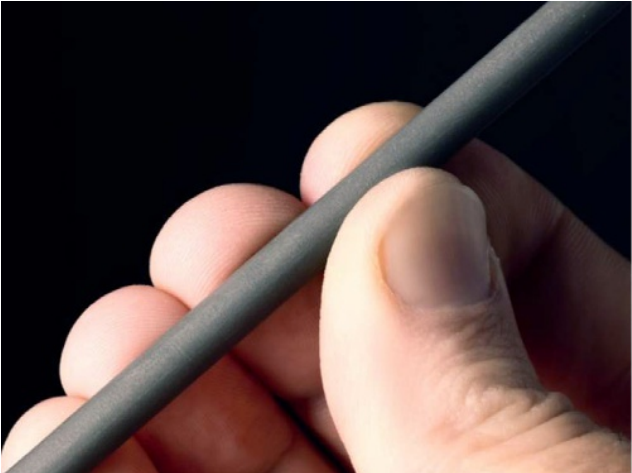
\includegraphics[width=0.5\linewidth]{bilder/Beispiel_Metallfilament.png}
        \caption[Beispiel für ein Metallfilament in Rohform] {Beispiel für ein Metallfilament in Rohform \autocite{MetalAdditiveMan}}
	\label{fig:FilamentBeispiel}
\end{figure}

Nachdem die gewünschte Kontur gefertigt ist, besteht sie weiterhin aus Metallpartikel gebunden mit Polymer. Damit dieses Polymer nun entweicht, wird es entbunden. Dazu wird das Bauteil in ein Bad aus Lösemittel für eine bestimmte Zeit gegeben. Dadurch löst sich das Polymer größtenteils und verlässt die Struktur. Übrig bleiben die Metallpartikel in der gewünschten Geometrie. Zuletzt wird das Bauteil in eine Sinteranlage gegeben. Dort wird es in Wasserstoffumgebung auf bis zu 1400C° erhitzt . Hierbei wird eine bestimmte Temperaturkurve mit Aufheiz-, Halte- und Abkühlphasen eingesetzt.\\
Dadurch verbinden sich die Metallpartikel auf molekularer Ebene und das fertige Metallteil ist fertig. Zu beachten ist jedoch, dass das Volumen und die Masse durch den Entbinder- und Sinterprozess schwindet, da das Polymer gelöst wird. \autocite{MetalAdditiveMan}

\begin{figure}[h]
	\centering
	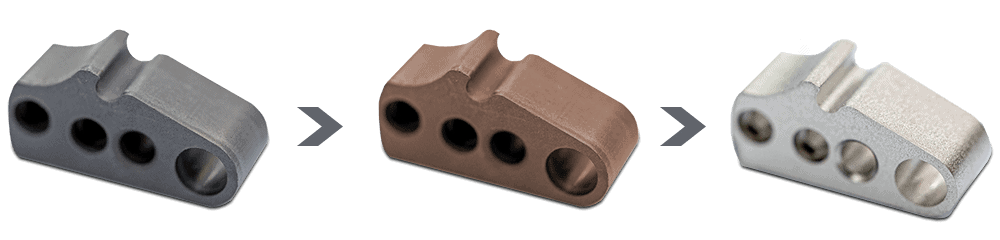
\includegraphics[width=0.8\linewidth]{bilder/img_gruenteil-braunteil-sinterteil.png}
        \caption[Der gesamte Prozess der Metallteilherstellung an einem Beispielteil dargestellt] {Der gesamte Prozess der Metallteilherstellung an einem Beispielteil dargestellt - von l. nach r. Grünteil; Braunteil, Sinterteil \autocite{junghans}}
	\label{fig:Prozess}
\end{figure}

In \autoref{fig:Prozess} ist der gesamte Prozess dargestellt. Links zu sehen ist das Bauteil, nachdem es aus dem 3D-Drucker entnommen wird. In der Mitte ist das entbundene Bauteil, in welchem der Polymer größtenteils gelöst und entfernt ist. Rechts im Bild zu sehen ist das Sinterbauteil, dies ist das fertige Bauteil.

\subsection{Arten des FDM-Verfahrens}
\label{sec:ArtenFDM}

FDM 3D-Drucker nutzen entweder einen Bowden-Extruder, oder einen Direktantrieb. Das Grundprinzip ist identisch, bei beiden Systemen fördert ein Elektromotor das Filament zum Hotend und damit zur Druckdüse. Die Verbindung von Elektromotor und Antriebsrad für das Filament wird Extruder genannt. Der Unterschied beider Verfahren ist die Lage dieses Extruders.

\begin{figure}[h]
	\centering
	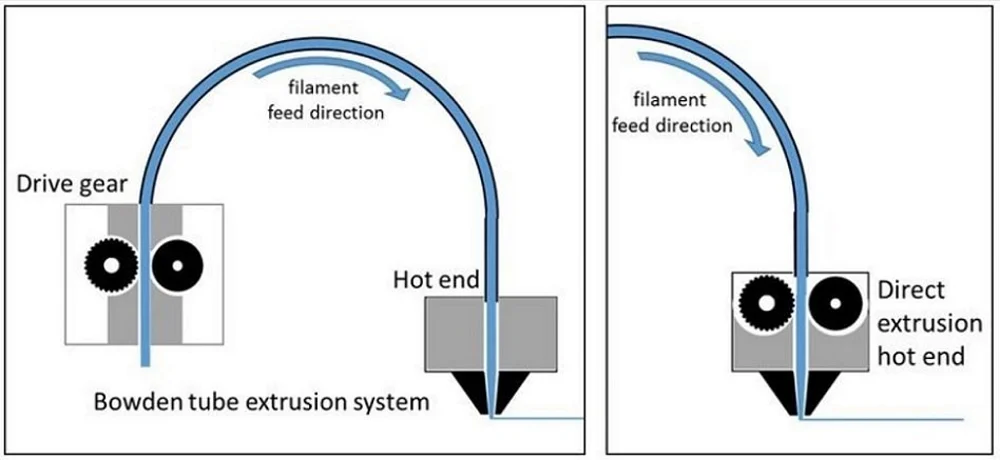
\includegraphics[width=0.8\linewidth]{bilder/img_BowdenvsDrirect.png}
        \caption[Schematische Darstellung von Bowden-Antrieb (links) und Direktantrieb (rechts)] {Schematische Darstellung von Bowden-Antrieb (links) und Direktantrieb (rechts) \autocite{facfox}}
	\label{fig:Verfahren}
\end{figure}

Wie in \autoref{fig:Verfahren} dargestellt, sitzt der Extruder beim Bowden-Extruder weit hinter der Düse. Das Filament wird vom Extruder durch einen Polytetrafluorethylen-Schlauch \textit{(PTFE)} und zum heißen Heizblock \textit{engl. Hotend} gedrückt. In dem Heizblock befindet sich die Druckdüse, durch die das aufgeheizte Filament extrudiert wird. Beim Direktextruder hingegen ist der Extruder unmittlebar vorm Hotend befestigt, dadurch wird das Filament vom PTFE-Schlauch direkt in den Extruder gepresst. Die Vor- und Nachteile sind hier aufgelistet:

\subsection*{Vorteile Direktextruder:}
\begin{itemize}
    \item Weniger Extrusionsprobleme: Der Extruder kann das Filament direkt zum Hotend fördern und muss es nicht durch ein Schlauch drücken.
    \item Kleinerer Motor notwendig: Aufgrund des kürzeren Abstands zwischen Extruder und Hotend wird weniger Drehmoment vom Motor benötigt.
    \item Mehr Auswahl an Filamenten: Sprödere Materialien, wie zum Beispiel Metallfilamente lassen sich drucken.
    \item Verbesserter Rückzug: der Extruder kann das Filament leichter zurückziehen, da er direkt über dem Hotend verbaut ist.
\end{itemize}

\subsection*{Nachteile Direktextruder:}
\begin{itemize}
    \item Höheres zu bewegendes Gewicht: Da der Extruder direkt am Druckkopf befestigt ist, muss er allen Bewegungen des Druckkopfes folgen. Dies sorgt für schlechtere dynamische Eigenschaften und Vibrationen
    \item Aufwändigere Wartung: Der Extruder ist am Druckkopf befestigt, welches eventuelle Wartungsarbeiten erschwert.
\end{itemize}

Für den Antrieb nach dem Bowden-Prinzip ergeben sich genau gespiegelte Vor- und Nachteile. \autocite{facfox}

\subsection{Lineare Vorschubtechnik}
\label{sec:LineareVorschub}

Die Lineare Vorschubregelung \textit{(engl. linear advance)}, ist eine Technik, die darauf abzielt, die Druckqualität und Geschwindigkeit beim FDM-Druck zu verbessern. Es sich dabei um einen algorithmischen Ansatz, der die Materialzufuhr während des Druckens in Echtzeit optimiert. Durch die Berücksichtigung der variablen Geschwindigkeiten und Beschleunigungen des Druckkopfes ermöglicht die Lineare Vorschubregelung eine präzisere Steuerung des Filamentflusses.
Die Lineare Vorschubregelung basiert auf der Idee, dass die Materialzufuhr nicht statisch ist, sondern dynamisch an die Bewegungen des Druckkopfes angepasst wird. Dieser Algorithmus betrachtet die Geschwindigkeitsänderungen des Druckkopfes und passt den Filamentvorschub linear an. Dies führt zu einer Reduzierung von Druckartefakten wie Überextrusion in Kurven oder Unterextrusion in geraden Abschnitten. \autocite{prusaLinearAdvance}

\begin{figure}[h]
	\centering
	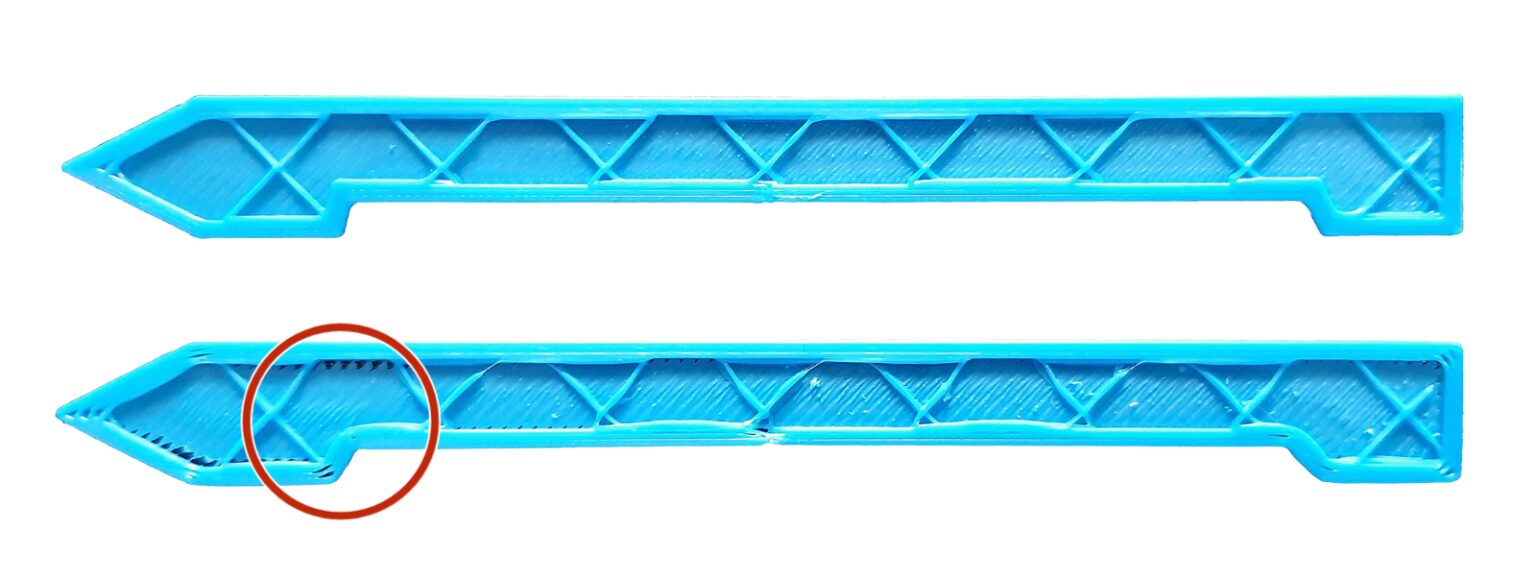
\includegraphics[width=0.8\linewidth]{bilder/img_linear-advance.jpeg}
        \caption[Darstellung lineare Vorschubregelung] {Darstellung lineare Vorschubregelung - oben: gutes Druckergebnis; unten: Artefakte durch falsche Einstellung von linearer Vorschubregelung \autocite{prusaLinearAdvance}}
	\label{fig:linearadvance}
\end{figure}